\documentclass[crop,tikz,border=8pt]{standalone}
\usepackage[utf8]{inputenc}
\usepackage[T1]{fontenc}
\usetikzlibrary{arrows.meta,calc}

\begin{document}
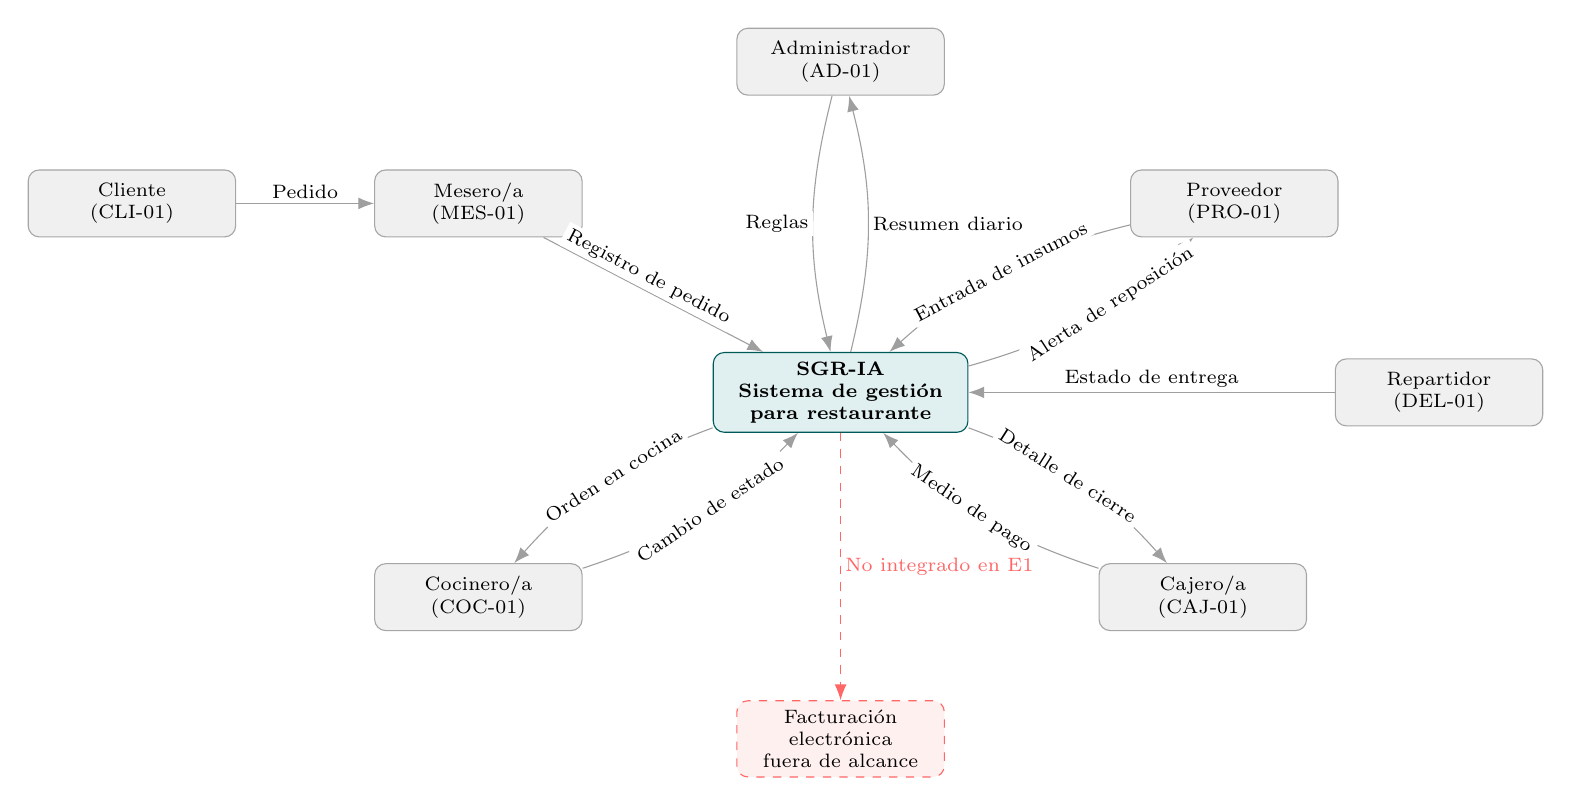
\begin{tikzpicture}[
  sys/.style={draw=teal!70!black,fill=teal!12,rounded corners,align=center,
              text width=3.0cm,minimum height=1.0cm,font=\scriptsize\bfseries},
  ext/.style={draw=gray!70,fill=gray!12,rounded corners,align=center,
              text width=2.4cm,minimum height=0.85cm,font=\scriptsize},
  arr/.style={-{Latex[length=2mm]},draw=gray!75,font=\scriptsize},
  lbl/.style={fill=white,inner sep=1.5pt,font=\scriptsize}
]
\node[sys] (sys) at (0,0) {SGR-IA\\Sistema de gestión para restaurante};
\node[ext] (adm) at (0,4.2) {Administrador\\(AD-01)};
\node[ext] (cli) at (-9.0,2.4) {Cliente\\(CLI-01)};
\node[ext] (mes) at (-4.6,2.4) {Mesero/a\\(MES-01)};
\node[ext] (coc) at (-4.6,-2.6) {Cocinero/a\\(COC-01)};
\node[ext] (pro) at (5.0,2.4) {Proveedor\\(PRO-01)};
\node[ext] (del) at (7.6,0) {Repartidor\\(DEL-01)};
\node[ext] (caj) at (4.6,-2.6) {Cajero/a\\(CAJ-01)};
\node[ext,draw=red!60,fill=red!6,dashed] (sri) at (0,-4.4) {Facturación electrónica\\fuera de alcance};

\draw[arr] (cli) -- node[lbl,above] {Pedido} (mes);
\draw[arr] (mes) -- node[lbl,above,sloped,pos=0.45] {Registro de pedido} (sys);
\draw[arr] (sys) to[bend right=14] node[lbl,sloped,pos=0.45] {Orden en cocina} (coc);
\draw[arr] (coc) to[bend right=14] node[lbl,sloped,pos=0.55] {Cambio de estado} (sys);
\draw[arr] (sys) to[bend left=14] node[lbl,sloped,pos=0.45] {Detalle de cierre} (caj);
\draw[arr] (caj) to[bend left=14] node[lbl,sloped,pos=0.55] {Medio de pago} (sys);
\draw[arr] (adm) to[bend right=14] node[lbl,left,pos=0.5] {Reglas} (sys);
\draw[arr] (sys) to[bend right=14] node[lbl,right,pos=0.5] {Resumen diario} (adm);
\draw[arr] (pro) to[bend right=14] node[lbl,sloped,pos=0.5] {Entrada de insumos} (sys);
\draw[arr] (sys) to[bend right=14] node[lbl,sloped,pos=0.6] {Alerta de reposición} (pro);
\draw[arr] (del) -- node[lbl,above,pos=0.5] {Estado de entrega} (sys);
\draw[arr,dashed,red!60] (sys) -- node[lbl,right] {No integrado en E1} (sri);
\end{tikzpicture}
\end{document}
